%Este trabalho está licenciado sob a Licença Atribuição-CompartilhaIgual 4.0 Internacional Creative Commons. Para visualizar uma cópia desta licença, visite http://creativecommons.org/licenses/by-sa/4.0/deed.pt_BR ou mande uma carta para Creative Commons, PO Box 1866, Mountain View, CA 94042, USA.

\section{Gráficos}\label{sec_graf}

A {\PYTHONmatplotlib} é uma biblioteca {\python} livre e gratuita para a visualização de dados. É muito utilizada para a criação de gráficos estáticos, animados ou iterativos. Aqui, vamos introduzir alguma de suas ferramentas básicas para gráficos.

Para utilizá-la, é necessário instalá-la. Pacotes de instalação estão disponíveis para os principais sistemas operacionais, consule a sua loja de {\it apps} ou \href{https://matplotlib.org/stable/users/installing.html}{Matplotlib Installation}. Para importá-la, usamos

\begin{lstlisting}
import matplotlib.pyplot as plt
\end{lstlisting}

\begin{obs}
  Se você está usando um console {\python} remoto, você pode querer adicionar a seguinte linha de comando para que os gráficos sejam visualizados no próprio console.

\begin{lstlisting}
%matplotlib inline
\end{lstlisting}

\end{obs}

\begin{figure}[h]
  \centering
  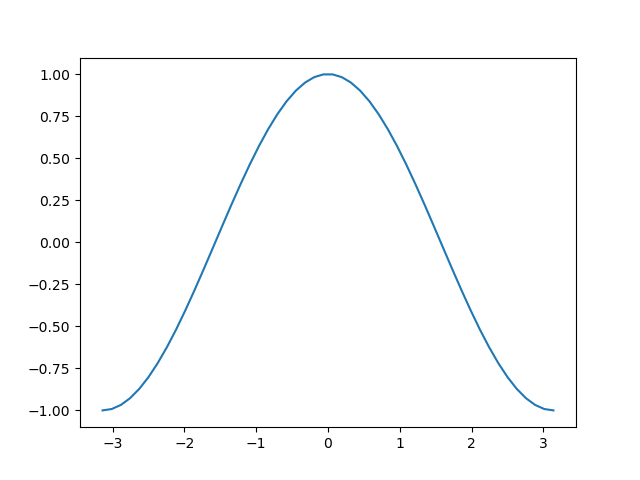
\includegraphics[width=0.7\textwidth]{./data/sen}
  \caption{Esboço do gráfico da função $y=\sen(x)$ no intervalo $[-\pi,\pi]$.}
  \label{fig:sen}
\end{figure}

Gráficos bidimensionais podem ser criados com a função {\PYTHONmatplotlibDOTpyplotDOTplot}\texttt{(x,y)}, onde \texttt{x} e \texttt{y} são \texttt{arrays} que fornecem os pontos cartesianos $(x_i, y_i)$ a serem plotados. Por exemplo,

\begin{lstlisting}
import matplotlib.pyplot as plt
x = np.linspace(-np.pi, np.pi)
y = np.cos(x)
plt.plot(x,y)
plt.show()
\end{lstlisting}

produz o seguinte esboço do gráfico da função $y=\sen(x)$ no intervalo $[-\pi,\pi]$. Consulte a Figura \ref{fig:sen}.


\begin{obs}
  Matplotlib é uma poderosa ferramenta para a visualização de gráficos. Consulte a galeria de exemplos no seu site oficial
  \begin{center}
    \url{https://matplotlib.org/stable/gallery/index.html}
  \end{center}
\end{obs}

\begin{exr}
  Crie um esboço do gráfico de cada uma das seguintes funções no intervalo indicado:
  \begin{enumerate}[a)]
  \item $y = \cos(x)$, $\left[0, 2\pi\right]$
  \item $y = x^2 - x + 1$, $[-2, 2]$
  \item $y = \tg\left(\frac{\pi}{2}x\right)$, $(-1, 1)$
  \end{enumerate}
\end{exr}
